% $Header: /Users/joseph/Documents/LaTeX/beamer/solutions/conference-talks/conference-ornate-20min.en.tex,v 90e850259b8b 2007/01/28 20:48:30 tantau $

\documentclass[xcolor={usenames,dvipsnames}]{beamer}

% This file is a solution template for:

% - Talk at a conference/colloquium.
% - Talk length is about 20min.
% - Style is ornate.



% Copyright 2004 by Till Tantau <tantau@users.sourceforge.net>.
%
% In principle, this file can be redistributed and/or modified under
% the terms of the GNU Public License, version 2.
%
% However, this file is supposed to be a template to be modified
% for your own needs. For this reason, if you use this file as a
% template and not specifically distribute it as part of a another
% package/program, I grant the extra permission to freely copy and
% modify this file as you see fit and even to delete this copyright
% notice. 


\mode<presentation>
{
  \usetheme{AnnArbor}
  % or ...

  \setbeamercovered{transparent}
  % or whatever (possibly just delete it)
 }

\usepackage[percent]{overpic}
\usepackage[english]{babel}
% or whatever

\usepackage[latin1]{inputenc}
% or whatever

\usepackage{times}
\usepackage[T1]{fontenc}
% Or whatever. Note that the encoding and the font should match. If T1
% does not look nice, try deleting the line with the fontenc.
%particles
\newcommand{\jpsi}{\rm J/$\psi$}
\newcommand{\psip}{$\psi^\prime$}
\newcommand{\jpsiDY}{\rm J/$\psi$\,/\,DY}
\newcommand{\chic}{$\chi_{\rm c}$}
\newcommand{\pip}{$\pi^{+}$}
\newcommand{\pim}{$\pi^{-}$}
\newcommand{\pizero}{$\pi^{0}$}
\newcommand{\kap}{K$^{+}$}
\newcommand{\kam}{K$^{-}$}
\newcommand{\pbar}{$\rm\overline{p}$}
\newcommand{\ccbar}{\ensuremath{\mathrm{c\overline{c}}}}
\newcommand{\bbbar}{\ensuremath{\mathrm{b\overline{b}}}}
\newcommand{\Dzero}{\ensuremath{\mathrm{D^{0}}}}
\newcommand{\Dzerobar}{\ensuremath{\mathrm{\overline{D}^{0}}}}
\newcommand{\Dpm}{\ensuremath{\mathrm{D^{\pm}}}}
\newcommand{\Ds}{\ensuremath{\mathrm{D_{s}^{\pm}}}}
\newcommand{\Dstar}{\ensuremath{\mathrm{D^{*\pm}}}}

%collision systems
\newcommand{\pp}{pp}
\newcommand{\pPb}{p--Pb}
\newcommand{\PbPb}{Pb--Pb}

%detectors
\newcommand{\ezdc}{$E_{\rm ZDC}$}

%units
\newcommand{\GeVc}{GeV/$c$}
\newcommand{\GeVcsq}{GeV/$c^2$}

%others
\newcommand{\degree}{$^{\rm o}$}
\newcommand{\s}{\ensuremath{\sqrt{s}}}
\newcommand{\snn}{\ensuremath{\sqrt{s_{\rm NN}}}}
\newcommand{\y}{\ensuremath{y}}
\newcommand{\pt}{\ensuremath{p_{\rm T}}}
\newcommand{\dedx}{d$E$/d$x$}
\newcommand{\dndy}{d$N$/d$y$}
\newcommand{\dndydpt}{${\rm d}^2N/({\rm d}y {\rm d}p_{\rm t})$}
\newcommand{\zpar}{\ensuremath{z_{||}}}
\newcommand{\zpargen}{\ensuremath{z_{||}^{\mathrm{part}}}}
\newcommand{\zpardet}{\ensuremath{z_{||}^{\mathrm{det}}}}
\newcommand{\ptchjet}{\ensuremath{p_{\mathrm{T,ch\, jet}}}}
\newcommand{\ptjet}{\ensuremath{p_{\mathrm{T,jet}}}}
\newcommand{\ptchjetgen}{\ensuremath{p_{\mathrm{T,ch\,jet}}^{\mathrm{part}}}}
\newcommand{\ptchjetdet}{\ensuremath{p_{\mathrm{T,ch\,jet}}^{\mathrm{det}}}}
\newcommand{\ptd}{\ensuremath{p_{\mathrm{T,D}}}}
\newcommand{\ptdgen}{\ensuremath{p_{\mathrm{T,D}}^{\mathrm{part}}}}
\newcommand{\ptddet}{\ensuremath{p_{\mathrm{T,D}}^{\mathrm{det}}}}
\newcommand{\antikt}{anti-\ensuremath{k_{\mathrm{T}}}}
\newcommand{\Antikt}{Anti-\ensuremath{k_{\mathrm{T}}}}
\newcommand{\kt}{\ensuremath{k_{\mathrm{T}}}}
\newcommand{\pthard}{\ensuremath{p_{\mathrm{T,hard}}}}

\AtBeginSection[]{
  \begin{frame}
  \vfill
  \centering
  \begin{beamercolorbox}[sep=8pt,center,shadow=true,rounded=true]{title}
    \usebeamerfont{title}\insertsectionhead\par%
  \end{beamercolorbox}
  \vfill
  \end{frame}
}

\title[D-tagged jets in \pp\ and \pPb\ collisions] % (optional, use only with long paper titles)
{D-tagged jets in \pp\ and \pPb\ collisions}

\author[Salvatore Aiola]% (optional, use only with lots of authors)
{Salvatore Aiola$^{1}$ \\
Ant\^onio C.O. da Silva$^{2,3}$ \\
Barbara A. Trzeciak$^{3}$ \\ 
\bigskip
on behalf of PAG-HFCJ}
% - Give the names in the same order as the appear in the paper.
% - Use the \inst{?} command only if the authors have different
%   affiliation.

\institute[Yale University] % (optional, but mostly needed)
{$^{1}$Yale University\\
$^{2}$University of S\~ao Paulo \\
$^{3}$Utrecht University}

\date[PWG-HF - Dec. 13th, 2016] % (optional, should be abbreviation of conference name)
{PWG-HF \\
December 13th, 2016}
% - Either use conference name or its abbreviation.
% - Not really informative to the audience, more for people (including
%   yourself) who are reading the slides online

\subject{High-Energy Physics}
% This is only inserted into the PDF information catalog. Can be left
% out. 



% If you have a file called "university-logo-filename.xxx", where xxx
% is a graphic format that can be processed by latex or pdflatex,
% resp., then you can add a logo as follows:

% \pgfdeclareimage[height=0.5cm]{university-logo}{university-logo-filename}
% \logo{\pgfuseimage{university-logo}}


% If you wish to uncover everything in a step-wise fashion, uncomment
% the following command: 

%\beamerdefaultoverlayspecification{<+->}


\begin{document}

\begin{frame}
  \titlepage
\end{frame}

\begin{frame}{Outline}
    \tableofcontents
 \end{frame}


% Structuring a talk is a difficult task and the following structure
% may not be suitable. Here are some rules that apply for this
% solution: 

% - Exactly two or three sections (other than the summary).
% - At *most* three subsections per section.
% - Talk about 30s to 2min per frame. So there should be between about
%   15 and 30 frames, all told.

% - A conference audience is likely to know very little of what you
%   are going to talk about. So *simplify*!
% - In a 20min talk, getting the main ideas across is hard
%   enough. Leave out details, even if it means being less precise than
%   you think necessary.
% - If you omit details that are vital to the proof/implementation,
%   just say so once. Everybody will be happy with that.

\section{Introduction}

\begin{frame}{Analysis Overview}
\begin{itemize}
\item Select D meson candidates using PID and topological cuts
\begin{itemize}
\item as in D meson spectra analysis
\end{itemize}
\item For each candidate reconstruct the jet using the \antikt\ algorithm
\begin{itemize}
\item replace D-meson daughters with D-meson 4-momentum
\item use \kt\ algorithm to estimate the background (\pPb)
\end{itemize}
\item Invariant mass analysis to extract the signal
\begin{itemize}
\item invariant mass fits in bins of \ptjet, or
\item Side-Band (SB) \ptjet-spectra subtraction (in bins of \ptd)
\item  efficiency correction applied at this step as a \ptd-dependent weight
\end{itemize}
\item B feed-down subtraction using a POWHEG+PYTHIA simulation
\item Unfolding using detector response matrix from PYTHIA6+GEANT3 simulation
\item Datasets:
\begin{itemize}
\item \pp\ at $\s=7$~TeV: LHC10b,c,d,e pass4 (312 M events)
\item \pPb\ at $\s=5.02$~TeV: LHC13b,c pass2 (98 M events)
\end{itemize}
\end{itemize}
\end{frame}

\section{\pp\ Analysis}
\subsection{Raw Yield Extraction}

\begin{frame}{Invariant Mass Fits in \ptjet\ bins}
\begin{center}
\begin{overpic}[width=.85\textwidth, trim=0 0 0 0, clip]{img/D0_Charged_R040_JetPtBins_DPt_20}
\end{overpic}
\end{center}
\vspace{-20pt}
\small
\begin{itemize}
\item Efficiency correction applied as a \ptd-dependent weight when filling the invariant mass plots
\end{itemize}
\end{frame}

\begin{frame}{Side-Band Subtraction}
\begin{center}
\begin{overpic}[width=.8\textwidth, trim=0 0 0 0, clip]{img/D0_Charged_R040_DPtBins_JetPt_5_30_SideBand_D0_Charged_R040_JetPtSpectrum_DPt_20_SideBand}
\end{overpic}
\end{center}
\vspace{-20pt}
\footnotesize
\begin{itemize}
\item Invariant mass fits (in bins of \ptd) determine position and width of the mass peak
\item Background normalization is $B_{\rm fit}/B_{\rm SB}$: $B_{\rm fit}$ = bkg. under the peak ($2\sigma_{\rm fit}$) from fit and
$B_{\rm SB}$ = integral of the SB ($4\sigma_{\rm fit}<|m-m_{\rm fit}|<8\sigma_{\rm fit}$)
\end{itemize}
\end{frame}

\begin{frame}{Side-Band Spectra}
\begin{columns}
\column{.28\textwidth}
\begin{overpic}[width=\textwidth, trim=0 0 380 0, clip]{img/D0_Charged_R040_JetPtSpectrum_DPt_20_SideBand_BkgVsSig}
\end{overpic}
\column{.28\textwidth}
\begin{overpic}[width=\textwidth, trim=380 0 0 0, clip]{img/D0_Charged_R040_JetPtSpectrum_DPt_20_SideBand_BkgVsSig}
\end{overpic}
\column{.44\textwidth}
\begin{center}
\vspace{-10pt}
\tiny \sffamily
$2.0 < \ptd < 30.0$~\GeVc

\begin{overpic}[width=.8\textwidth, trim=0 0 0 0, clip]{img/D0_Charged_R040_JetPtSpectrum_DPt_20_SideBand_TotalBkgVsSig}
\end{overpic}
\end{center}
\footnotesize
\vspace{-20pt}
\begin{itemize}
\item \ptjet\ spectra scaled by a \ptd-dependent efficiency correction factor
\item Sum together all the \ptd\ bins
\end{itemize}
\end{columns}
\begin{itemize}
\item \textcolor{BrickRed}{SB} jet spectra ($4\sigma_{\rm fit}<|m-m_{\rm fit}|<8\sigma_{\rm fit}$) \textcolor{ForestGreen}{subtracted} from \textcolor{NavyBlue}{peak region} ($|m-m_{\rm fit}|<2\sigma_{\rm fit}$)
\end{itemize}
\end{frame}

\begin{frame}{Comparison of the two methods}
\begin{columns}
\column{.50\textwidth}
\begin{overpic}[width=\textwidth, trim=0 0 0 0, clip]{img/D0_Charged_R040_jet_pt_SpectraComparison}
\end{overpic}
\column{.50\textwidth}
\begin{overpic}[width=\textwidth, trim=0 0 0 0, clip]{img/D0_Charged_R040_jet_pt_SpectraComparison_Ratio}
\end{overpic}
\end{columns}
\begin{itemize}
\item The two methods give consistent results
\item Discrepancies are well within statistical precision -- albeit fluctuations are partially correlated
\end{itemize}
\end{frame}

\subsection{B feed-down correction}

\begin{frame}{B feed-down correction}

\begin{columns}
\column{.50\textwidth}
\begin{overpic}[width=\textwidth, trim=0 0 0 0, clip]{img/D0_Charged_R040_JetPtSpectrum_DPt_20_SideBand_FDCorrection}
\end{overpic}
\column{.50\textwidth}
\begin{overpic}[width=\textwidth, trim=0 0 0 0, clip]{img/D0_Charged_R040_JetPtSpectrum_DPt_20_SideBand_FDCorrection_Ratio}
\end{overpic}
\end{columns}
{\tiny
$\textcolor{NavyBlue}{N^{\rm c\rightarrow\Dzero}_{\rm det}(\ptchjet)} = N^{\rm c,b\rightarrow\Dzero}_{\rm raw}(\ptchjet) - 
\textcolor{BrickRed}{R_{\rm det}^{\rm b\rightarrow\Dzero}(\ptchjet) \otimes \sum_{\ptd} \frac{\epsilon^{\rm b\rightarrow\Dzero}(\ptd)}{\epsilon^{\rm c\rightarrow\Dzero}(\ptd)} N^{\rm b\rightarrow\Dzero}_{\rm POWHEG}(\ptd,\ptchjet)}$
}
\small
\begin{itemize}
\item B Feed-Down (FD) spectrum is estimated with a POWHEG+PYTHIA6 simulation (scaled by the luminosity)
\item Weighted by the ratio of the prompt and non-prompt \Dzero\ reconstruction efficiencies and smeared using detector response
\item Subtracted from the measured yield before unfolding
\end{itemize}
\vspace{-5pt}
{\tiny
Note: no normalization is applied and not divided by the bin width, these are counts weighted by the reconstruction efficiency
}

\end{frame}

\begin{frame}{FD \& Efficiency vs. \ptchjet\ and \ptd}
\begin{columns}
\column{.50\textwidth}
\begin{overpic}[width=\textwidth, trim=0 0 0 0, clip]{img/BFeedDownVsPtJet_powheg_Full_R040_1478868679_1478869008_Ratio}
\end{overpic}
\column{.50\textwidth}
\begin{overpic}[width=\textwidth, trim=0 0 0 0, clip]{img/D0_Jet_AKTChargedR040_pt_scheme_JetPtDPtSpectrum_PartialEfficiency}
\end{overpic}
\end{columns}
\begin{itemize}
\item POWHEG+PYTHIA: Feed-Down fraction monotonically increases as a function of \ptchjet\ (left)
\item PYTHIA+GEANT3: Reconstruction efficiency largely independent of \ptchjet, for $5<\ptchjet<30$~\GeVc\ (right)
\end{itemize}
\end{frame}

\begin{frame}{Prompt vs. Non-Prompt Detector Response}
\begin{center}
\begin{overpic}[width=.8\textwidth, trim=0 0 0 0, clip]{img/DetectorJetPtResolutionComparison}
\end{overpic}
\end{center}
\vspace{-20pt}
\small
\begin{itemize}
\item Momentum resolution as a function of \ptchjet
\item Significantly different response for b~$\rightarrow$~\Dzero (blue) compared c~$\rightarrow$~\Dzero (red)
\end{itemize}
\end{frame}

\begin{frame}{Smear w/ b~$\rightarrow$~\Dzero, unfold w/ c~$\rightarrow$~\Dzero}
\begin{columns}
\column{.50\textwidth}
\begin{overpic}[width=\textwidth, trim=0 0 0 0, clip]{img/FD_FoldUnfold_Comparison}
\end{overpic}
\column{.50\textwidth}
\begin{overpic}[width=\textwidth, trim=0 0 0 0, clip]{img/FD_FoldUnfold_Comparison_Ratio}
\end{overpic}
\end{columns}
\begin{itemize}
\item Feed-Down spectrum smeared using b~$\rightarrow$~\Dzero\ response (blue)
\item Unfolded using c~$\rightarrow$~\Dzero\ response (red)
\item Sanity check: unfold using b~$\rightarrow$~\Dzero\ response (green)
\end{itemize}
\end{frame}

\subsection{Unfolding}

\begin{frame}{Unfolding}
\begin{columns}
\column{.50\textwidth}
\begin{overpic}[width=\textwidth, trim=0 0 0 0, clip]{img/InvMassFit_DPt_20_UnfoldingSummary_Bayes}
\end{overpic}
\column{.50\textwidth}
\begin{overpic}[width=\textwidth, trim=0 0 0 0, clip]{img/InvMassFit_DPt_20_UnfoldingSummary_Bayes_UnfoldedOverMeasured}
\end{overpic}
\end{columns}
\begin{itemize}
\item Very small correction (5-10\%), much smaller than the statistical uncertainty!
\item Correction is small because: good momentum resolution (track-only, D-meson requirement) and large bins
\end{itemize}
\end{frame}

\begin{frame}{Unfolding Systematics}
\begin{columns}
\column{.50\textwidth}
\begin{center}
\tiny
Method Comparison
\begin{overpic}[width=.8\textwidth, trim=0 0 0 0, clip]{img/InvMassFit_DPt_20_UnfoldingMethod_Ratio}
\end{overpic}\\
Bayesian Regularization
\begin{overpic}[width=.8\textwidth, trim=0 0 0 0, clip]{img/InvMassFit_DPt_20_UnfoldingRegularization_Bayes_PriorResponseTruth_Ratio}
\end{overpic}
\end{center}
\column{.50\textwidth}
\begin{center}
\tiny
Prior Choice \\
\begin{overpic}[width=.8\textwidth, trim=0 0 0 0, clip]{img/InvMassFit_DPt_20_UnfoldingPrior_Bayes_Ratio}
\end{overpic}
\end{center}
\vspace{-20pt}
\begin{itemize}
\scriptsize
\item Baseline: Bayesian
\begin{itemize}
\tiny
\item fast convergence
\item stable after 3 iterations
\item then $< 1$\% variations
\end{itemize}
\item Methods: bin-by-bin correction, SVD
\begin{itemize}
\tiny
\item equivalent results within few \%
\end{itemize}
\item Priors: PYTHIA and $\ptjet^{-a}$ with $a=3, 7$
\begin{itemize}
\tiny
\item no effect on the unfolding
\end{itemize}
\end{itemize}
\end{columns}
\end{frame}

\begin{frame}{Unfolding: Summary}
\begin{itemize}
\item Very small correction
\item Very robust against:
\begin{itemize}
\item method variation (Bayesian, SVD, Bin-By-Bin)
\item priors choice
\item regularization strength
\end{itemize}
\item Systematic uncertainty much smaller than statistical $\approx 20-50$~\%
\item No uncertainty quoted, or few \% based on MC closure tests
\end{itemize}
\end{frame}

\section{\pPb\ Analysis}

\subsection{Raw Yield Extraction}

\begin{frame}
\frametitle{Jet \pt\ spectra with Eff. Scaled vs. SB methods}

\begin{columns}[c] 

\column{5.5cm} 
\footnotesize{Jet $p_{T}$ from data}
\begin{minipage}{1.\linewidth}
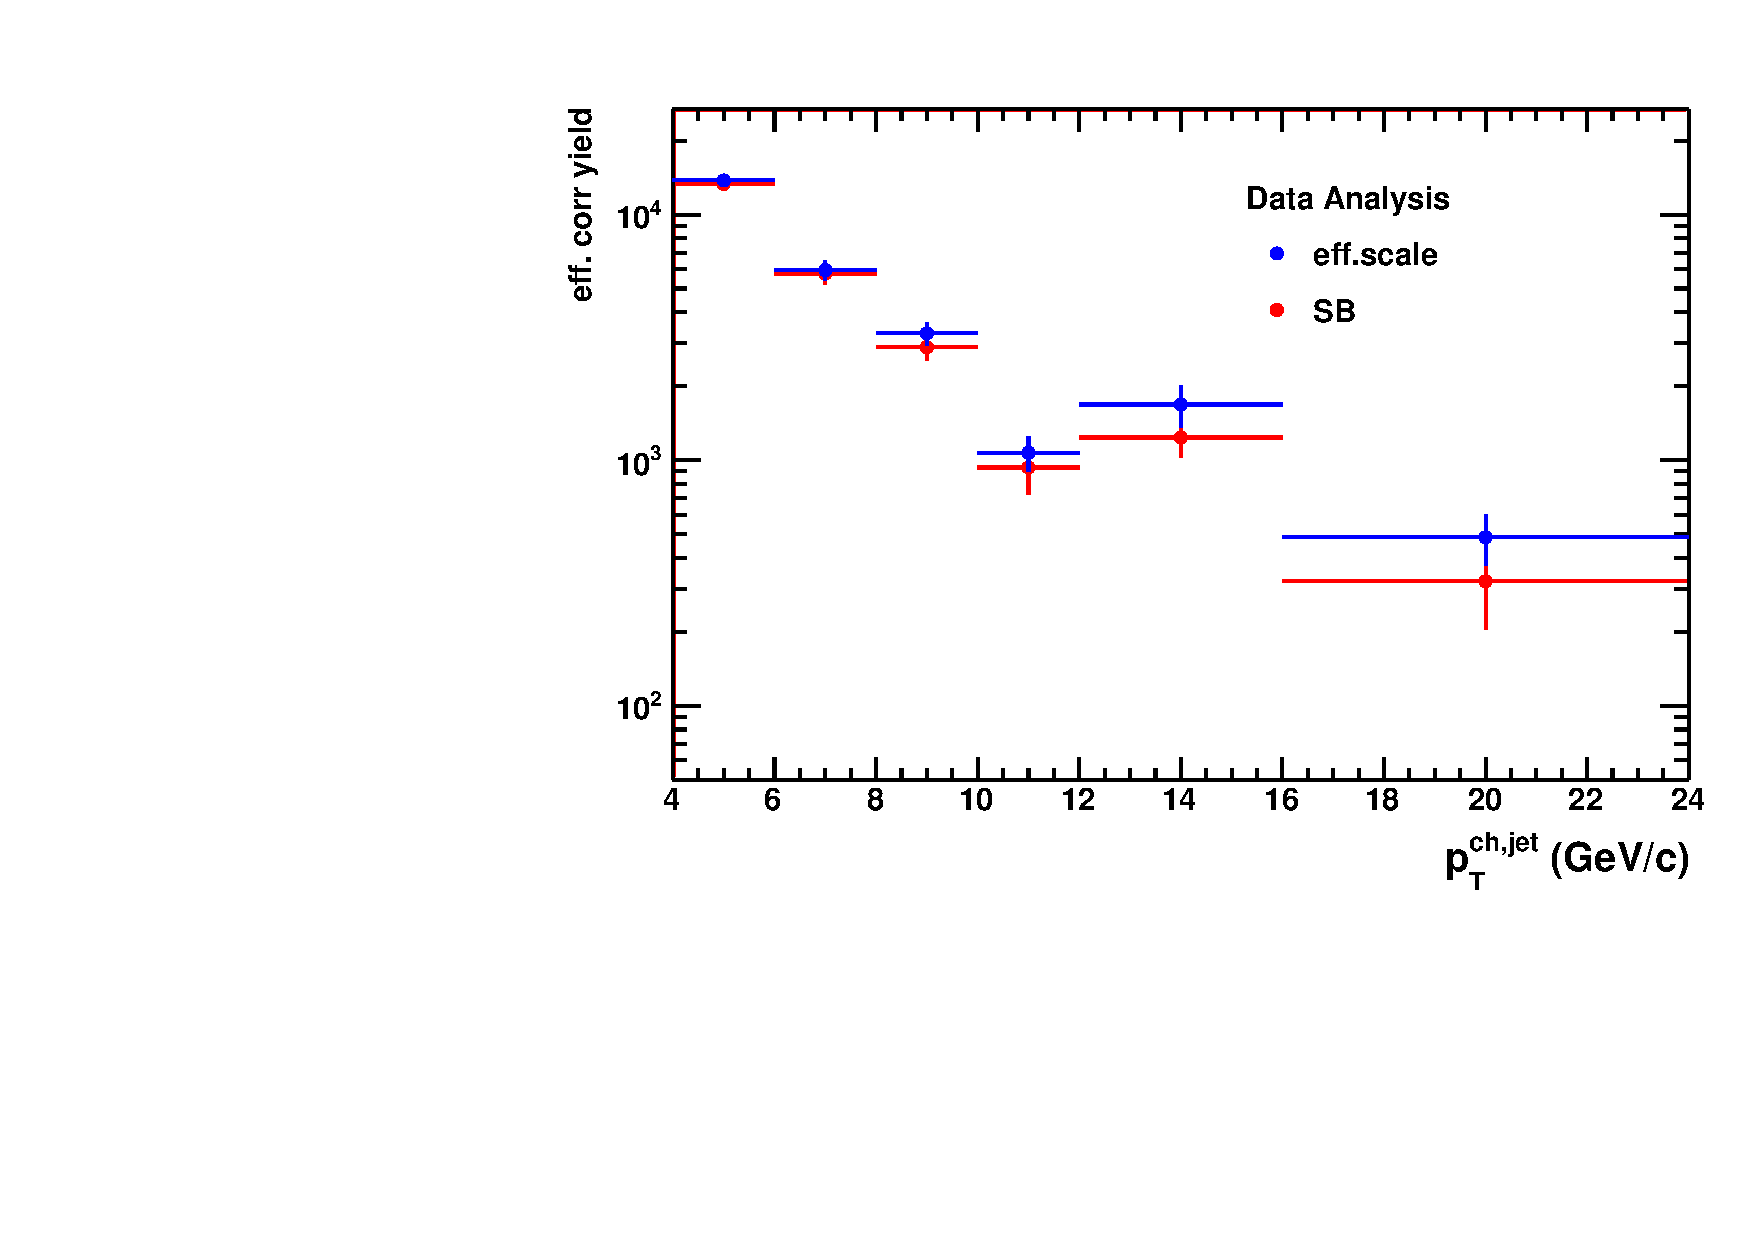
\includegraphics[width=0.95\linewidth]{img/rawYieldpPb/jetPtComparison_Data.pdf}
\end{minipage}
\begin{minipage}{1.\linewidth}
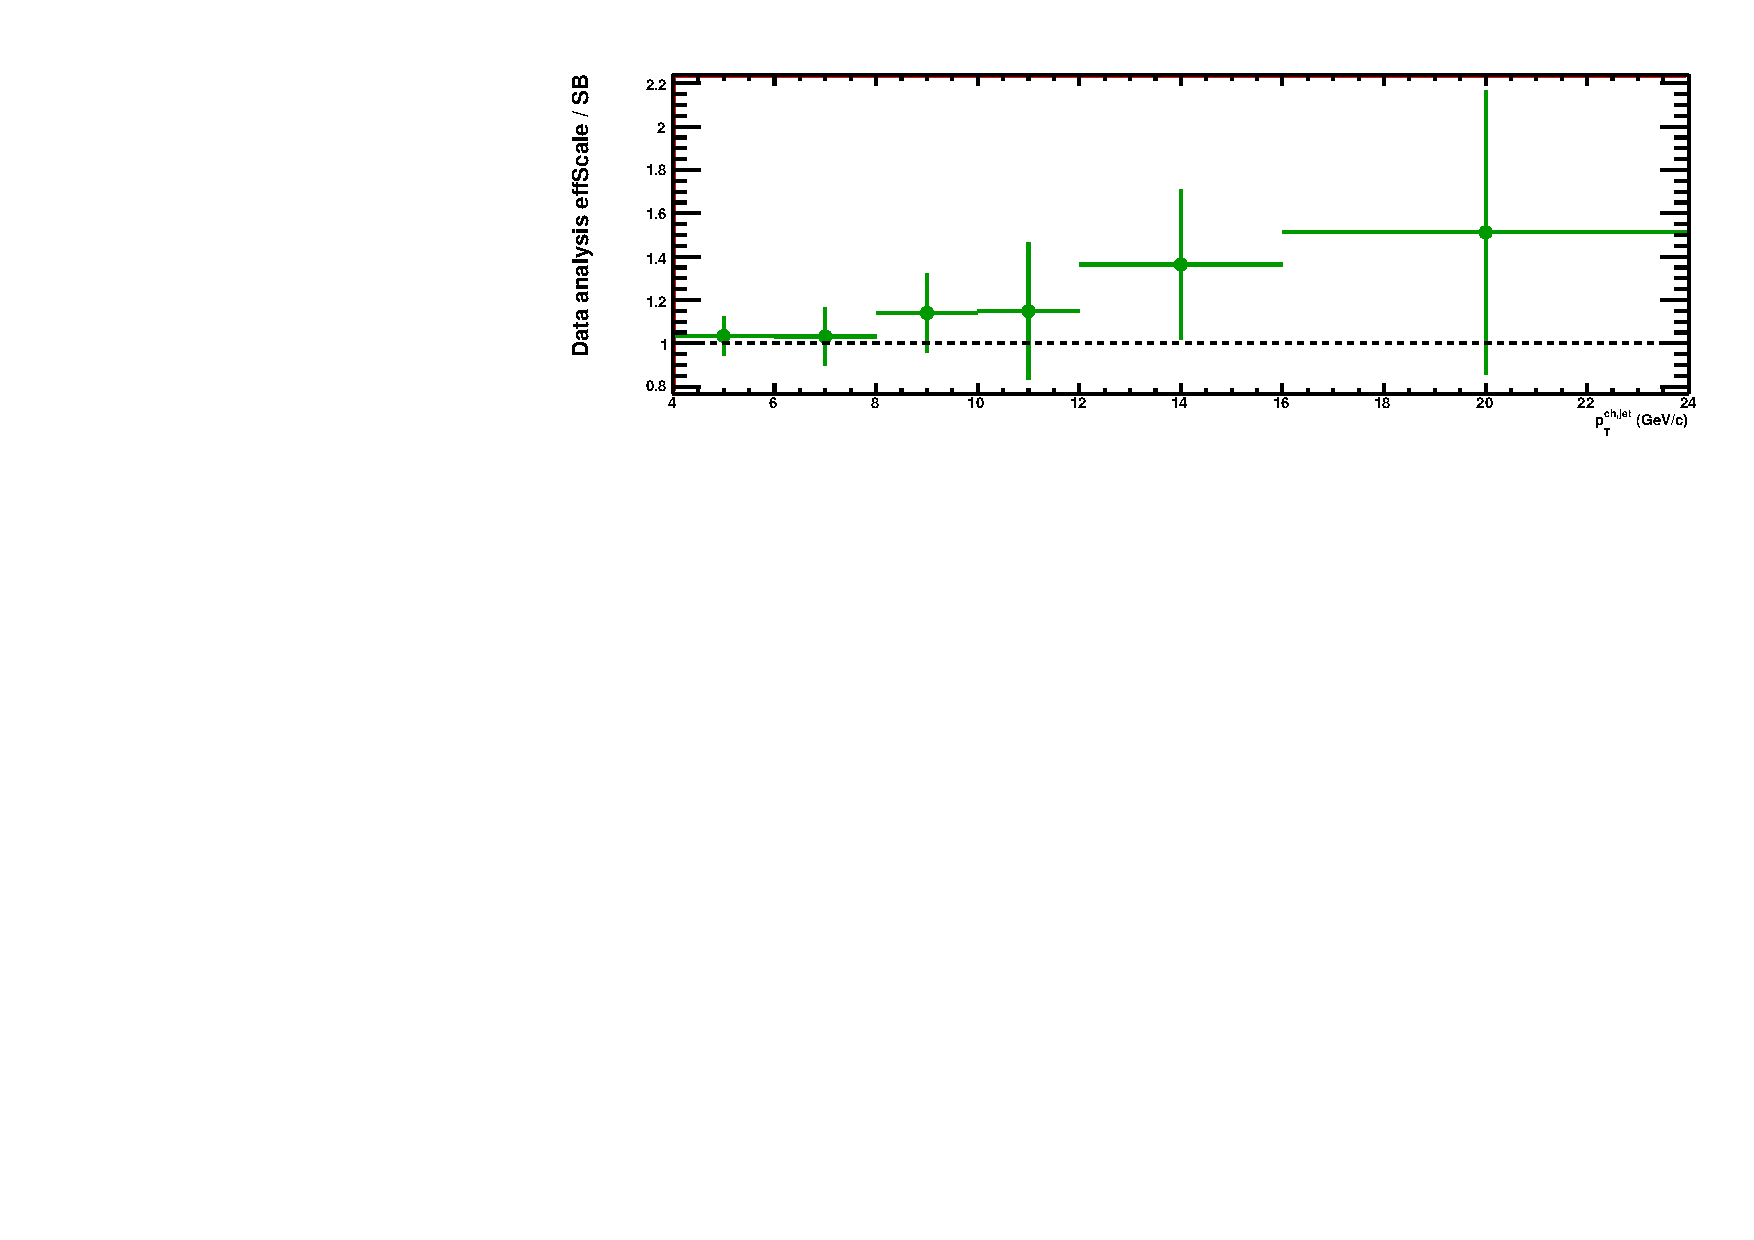
\includegraphics[width=0.95\linewidth]{img/rawYieldpPb/DataRatio.pdf}
\end{minipage}

\column{5.5cm} 
\footnotesize{statistical uncertainties}
\begin{minipage}{1.\linewidth}
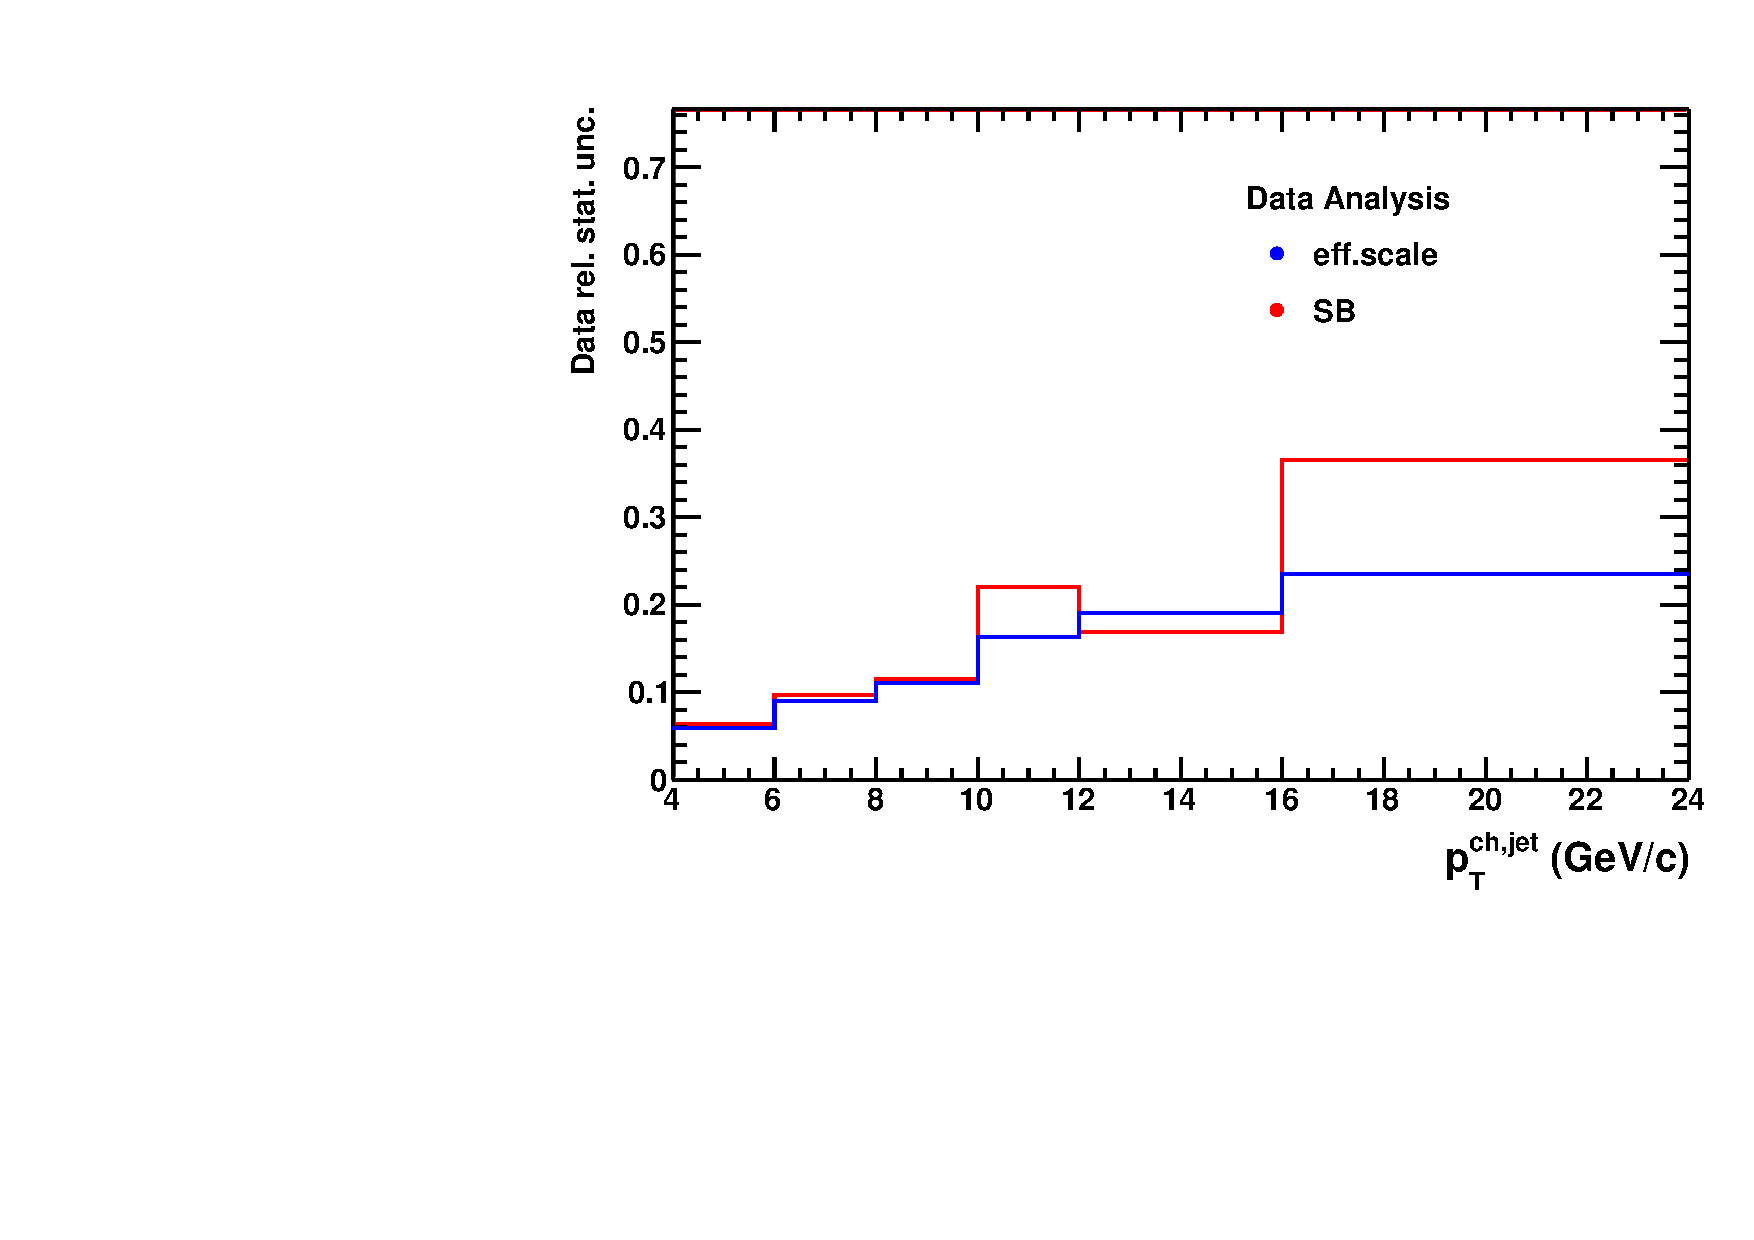
\includegraphics[width=0.95\linewidth]{img/rawYieldpPb/DataStatUnc.pdf}
\end{minipage}
	
\end{columns}

Difference due to fluctuation on the yield extraction (stat + syst effect), see next slides

\end{frame}

\subsection{Raw Yield Extraction Uncertainty}

\begin{frame}
\frametitle{Jet \pt\ spectra: average of variations}

\begin{columns}[c] 

\column{5.5cm} 
\footnotesize{Side-band method}
\begin{minipage}{1.\linewidth}
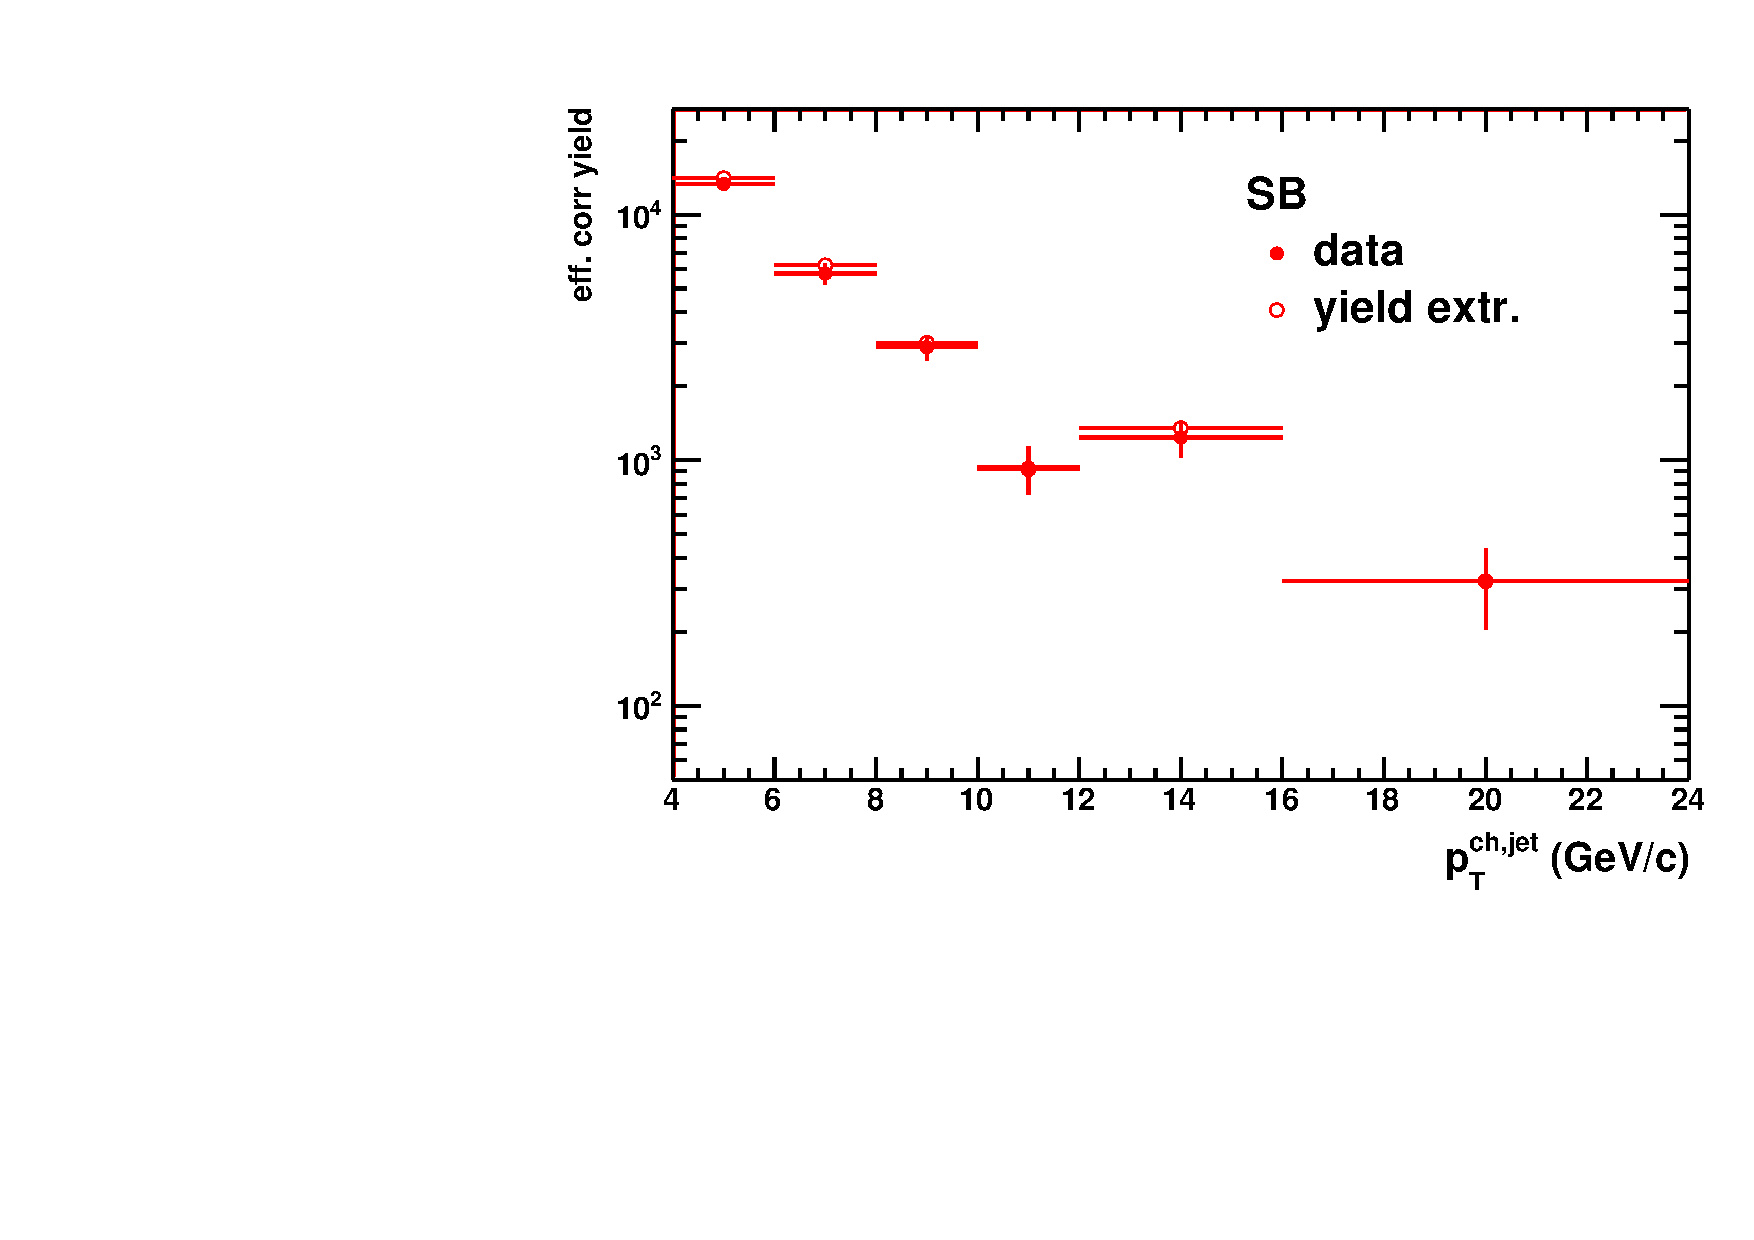
\includegraphics[width=0.95\linewidth]{img/rawYieldpPb/jetPtComparison_DataMVariation_SB.pdf}
\end{minipage}
\begin{minipage}{1.\linewidth}
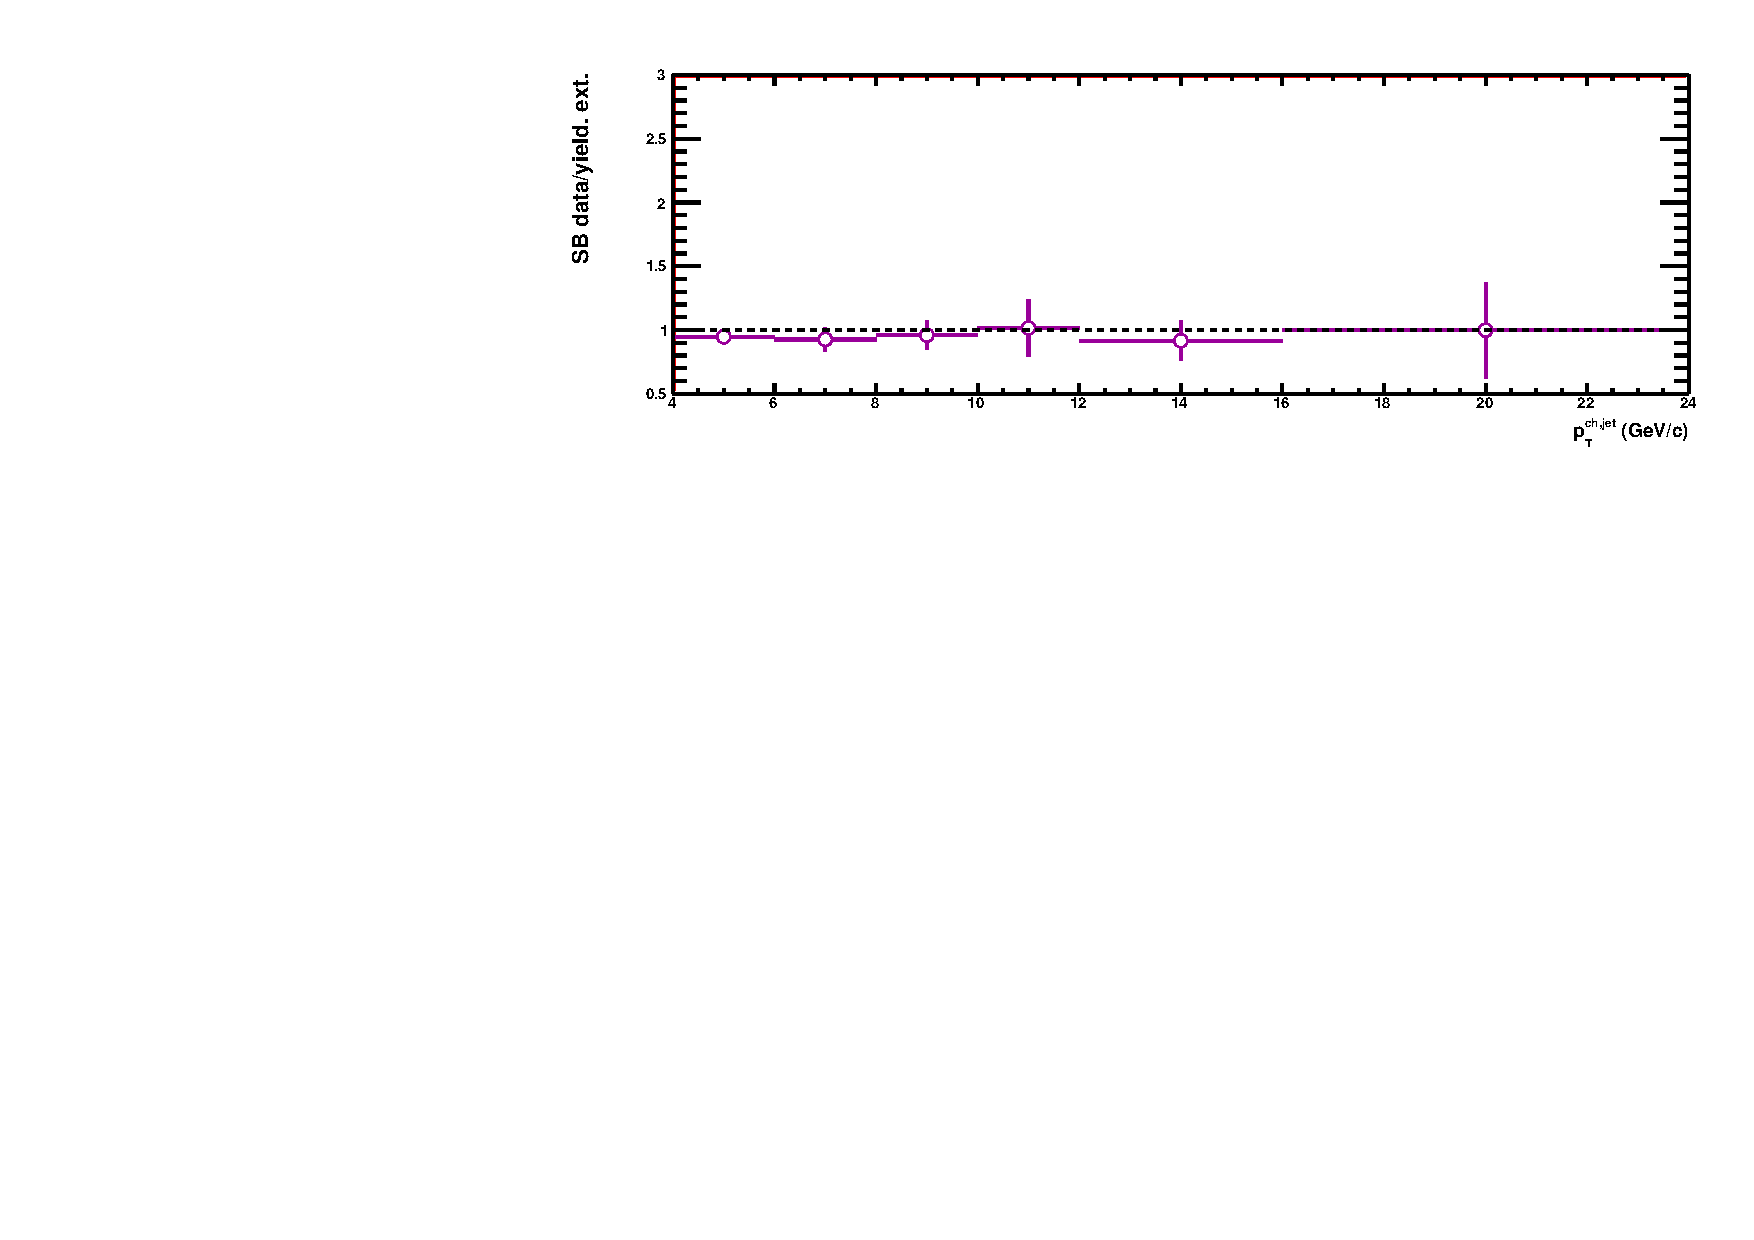
\includegraphics[width=0.95\linewidth]{img/rawYieldpPb/SBRatio.pdf}
\end{minipage}

\column{5.5cm} 
\footnotesize{efficiency scale method}
\begin{minipage}{1.\linewidth}
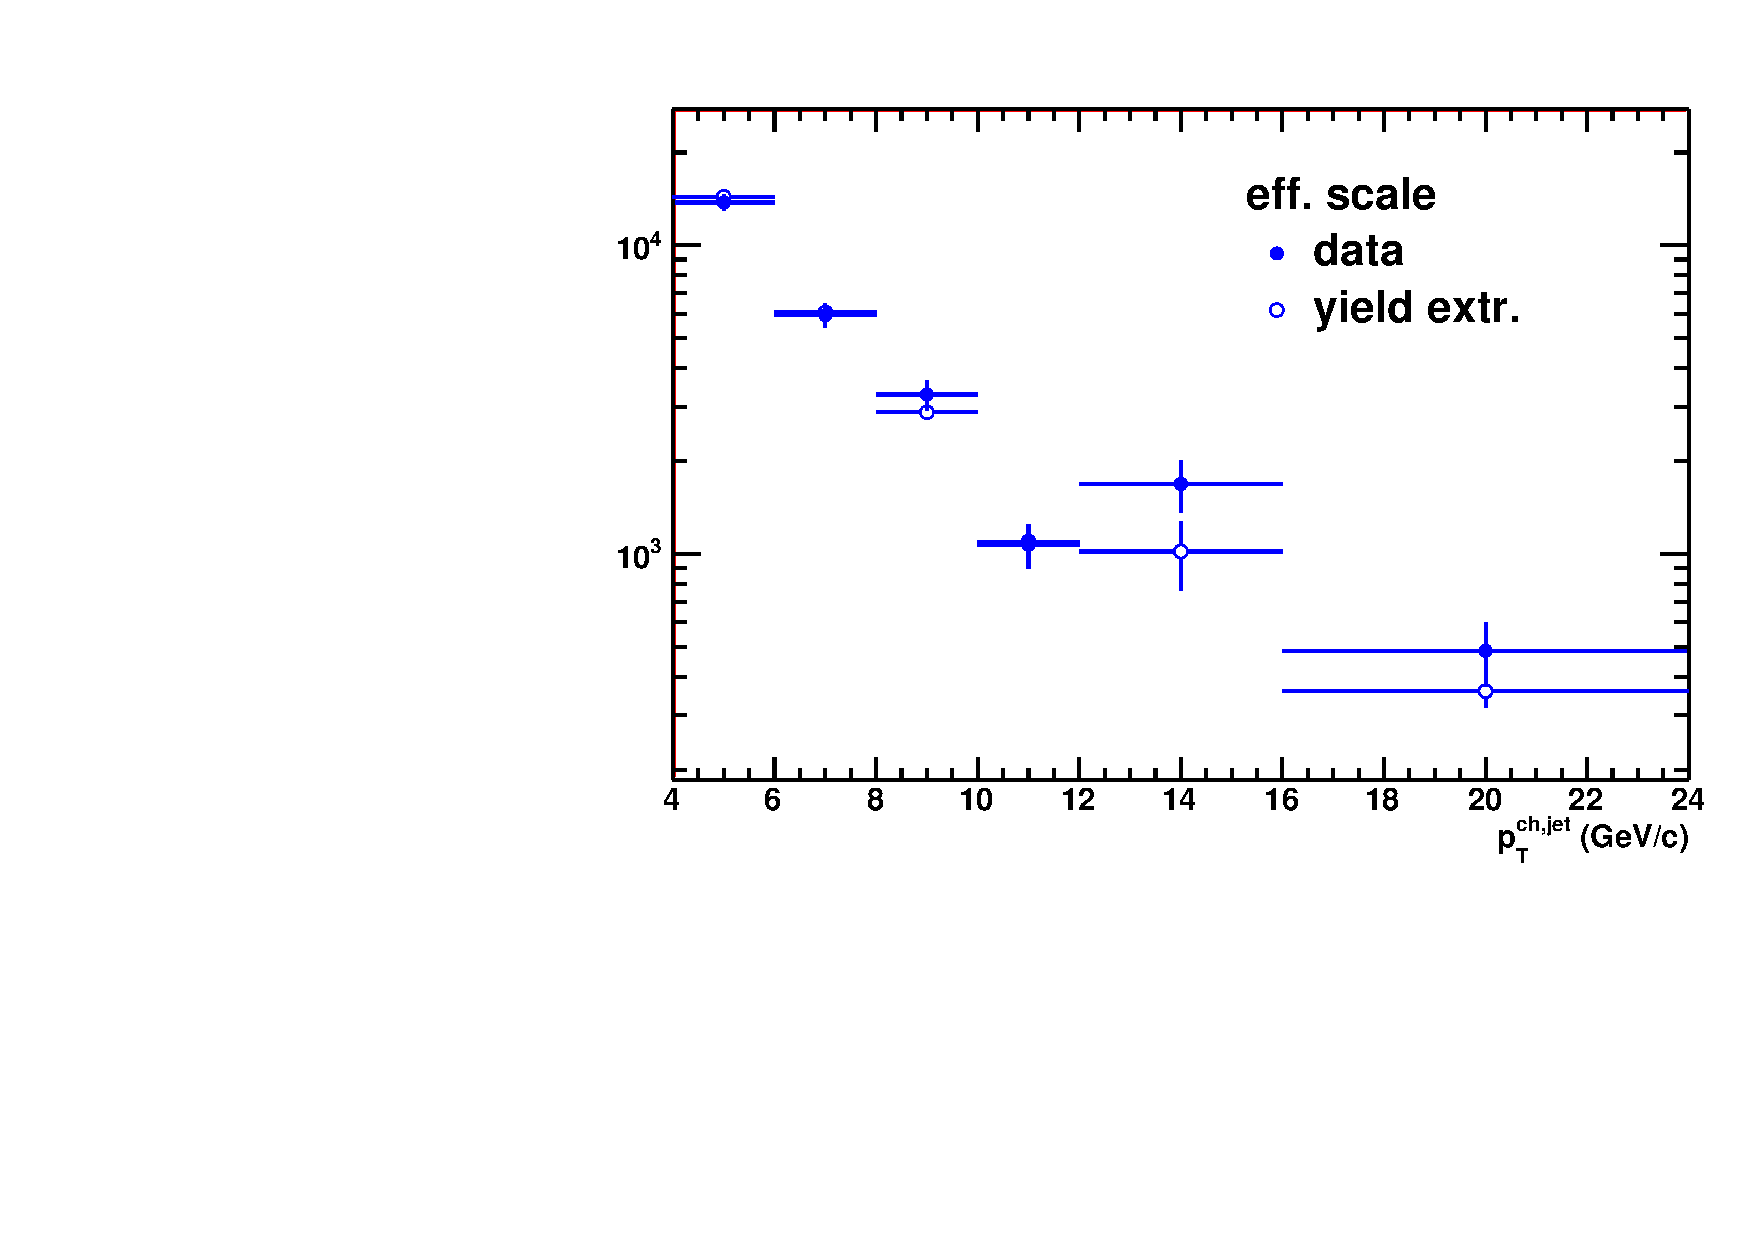
\includegraphics[width=0.95\linewidth]{img/rawYieldpPb/jetPtComparison_DataMVariation_effScale.pdf}
\end{minipage}
\begin{minipage}{1.\linewidth}
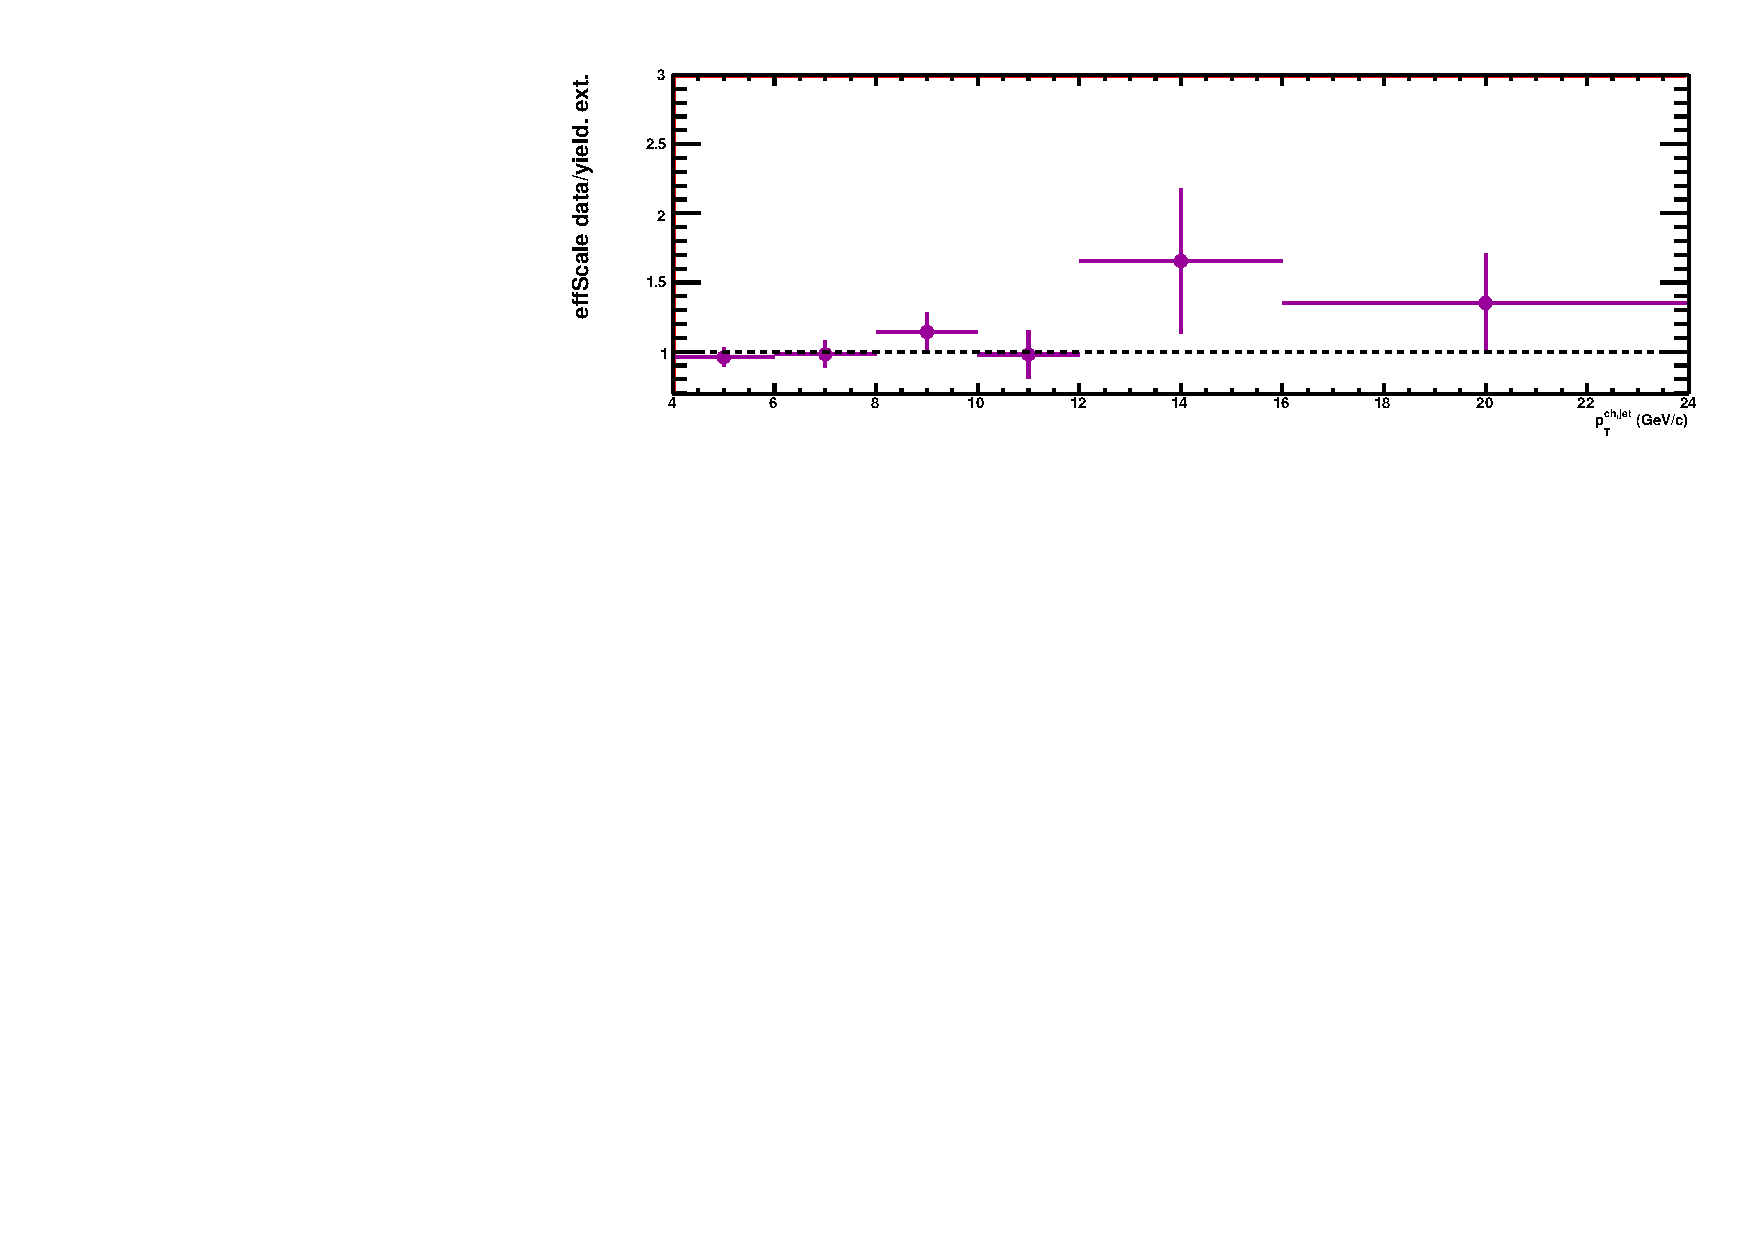
\includegraphics[width=0.95\linewidth]{img/rawYieldpPb/EffScaleRatio.pdf}
\end{minipage}
	
\end{columns}
\end{frame}

\begin{frame}
\frametitle{Systematic Uncertainty}

Central values of the jet \pt\ distributions from the yield variation procedure.
\vspace{2pt}
\begin{columns}[c] 

\column{5.5cm} 
\footnotesize{central yields}
\begin{minipage}{1.\linewidth}
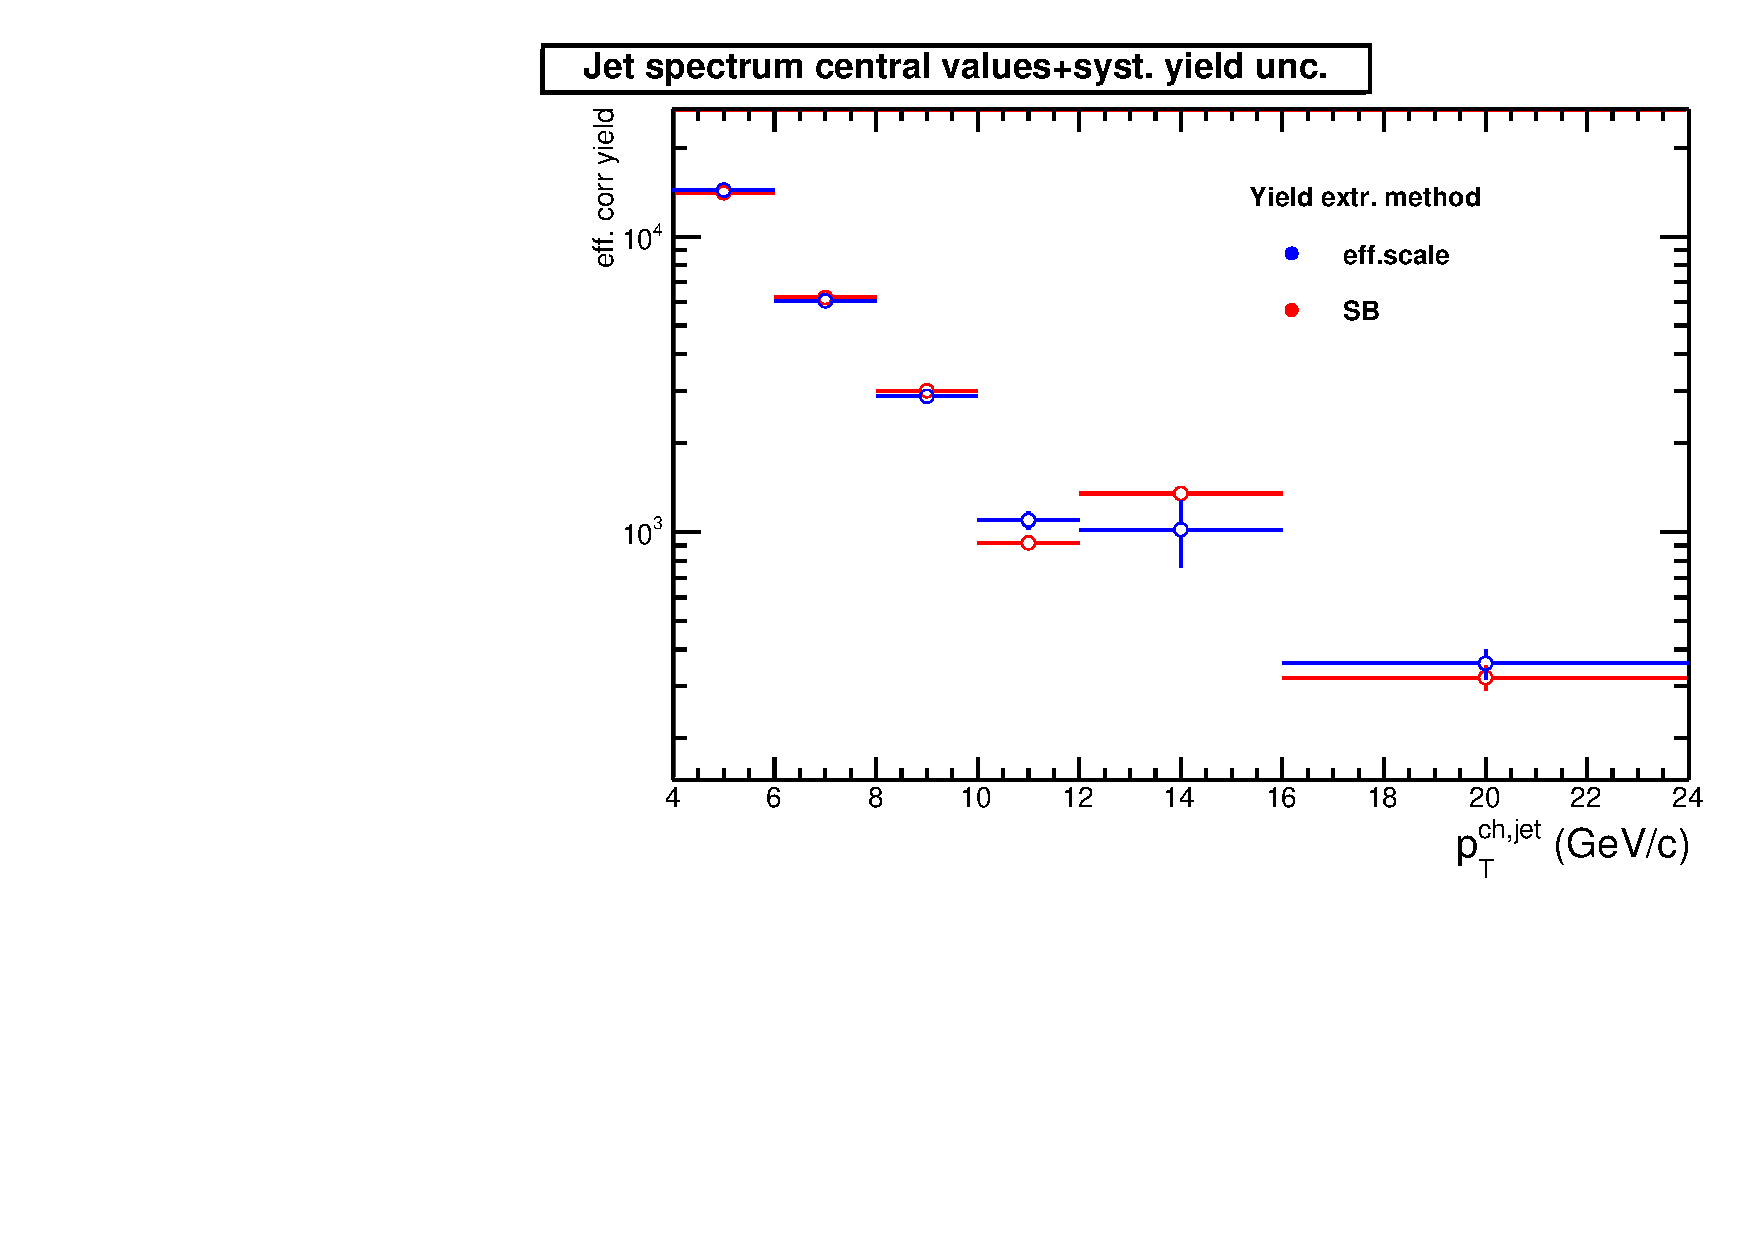
\includegraphics[width=0.95\linewidth]{img/rawYieldpPb/jetPtComparison_YieldExtractionCentral.pdf}
\end{minipage}
\begin{minipage}{1.\linewidth}
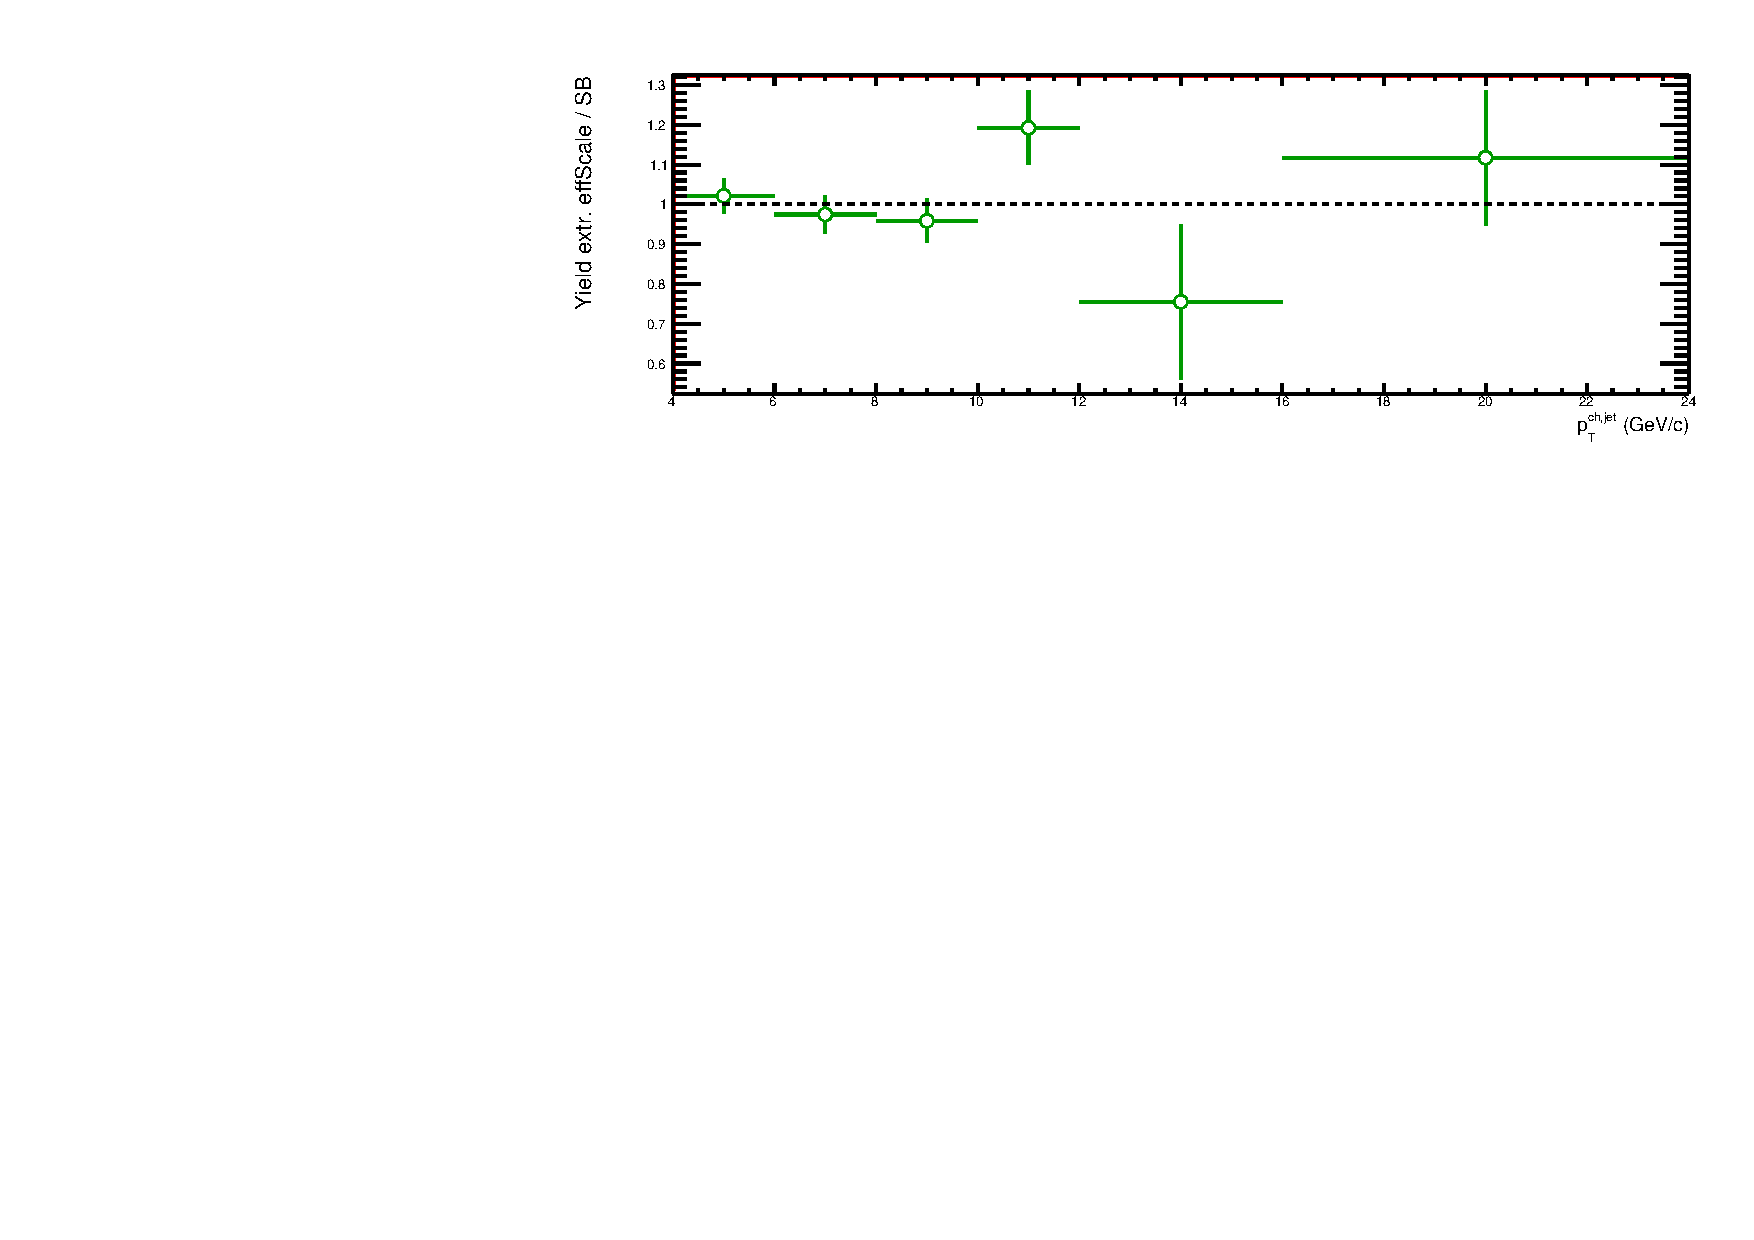
\includegraphics[width=0.95\linewidth]{img/rawYieldpPb/YieldExtractionRatio.pdf}
\end{minipage}

\column{5.5cm} 
\footnotesize{relative systematic uncertainties}
\begin{minipage}{1.\linewidth}
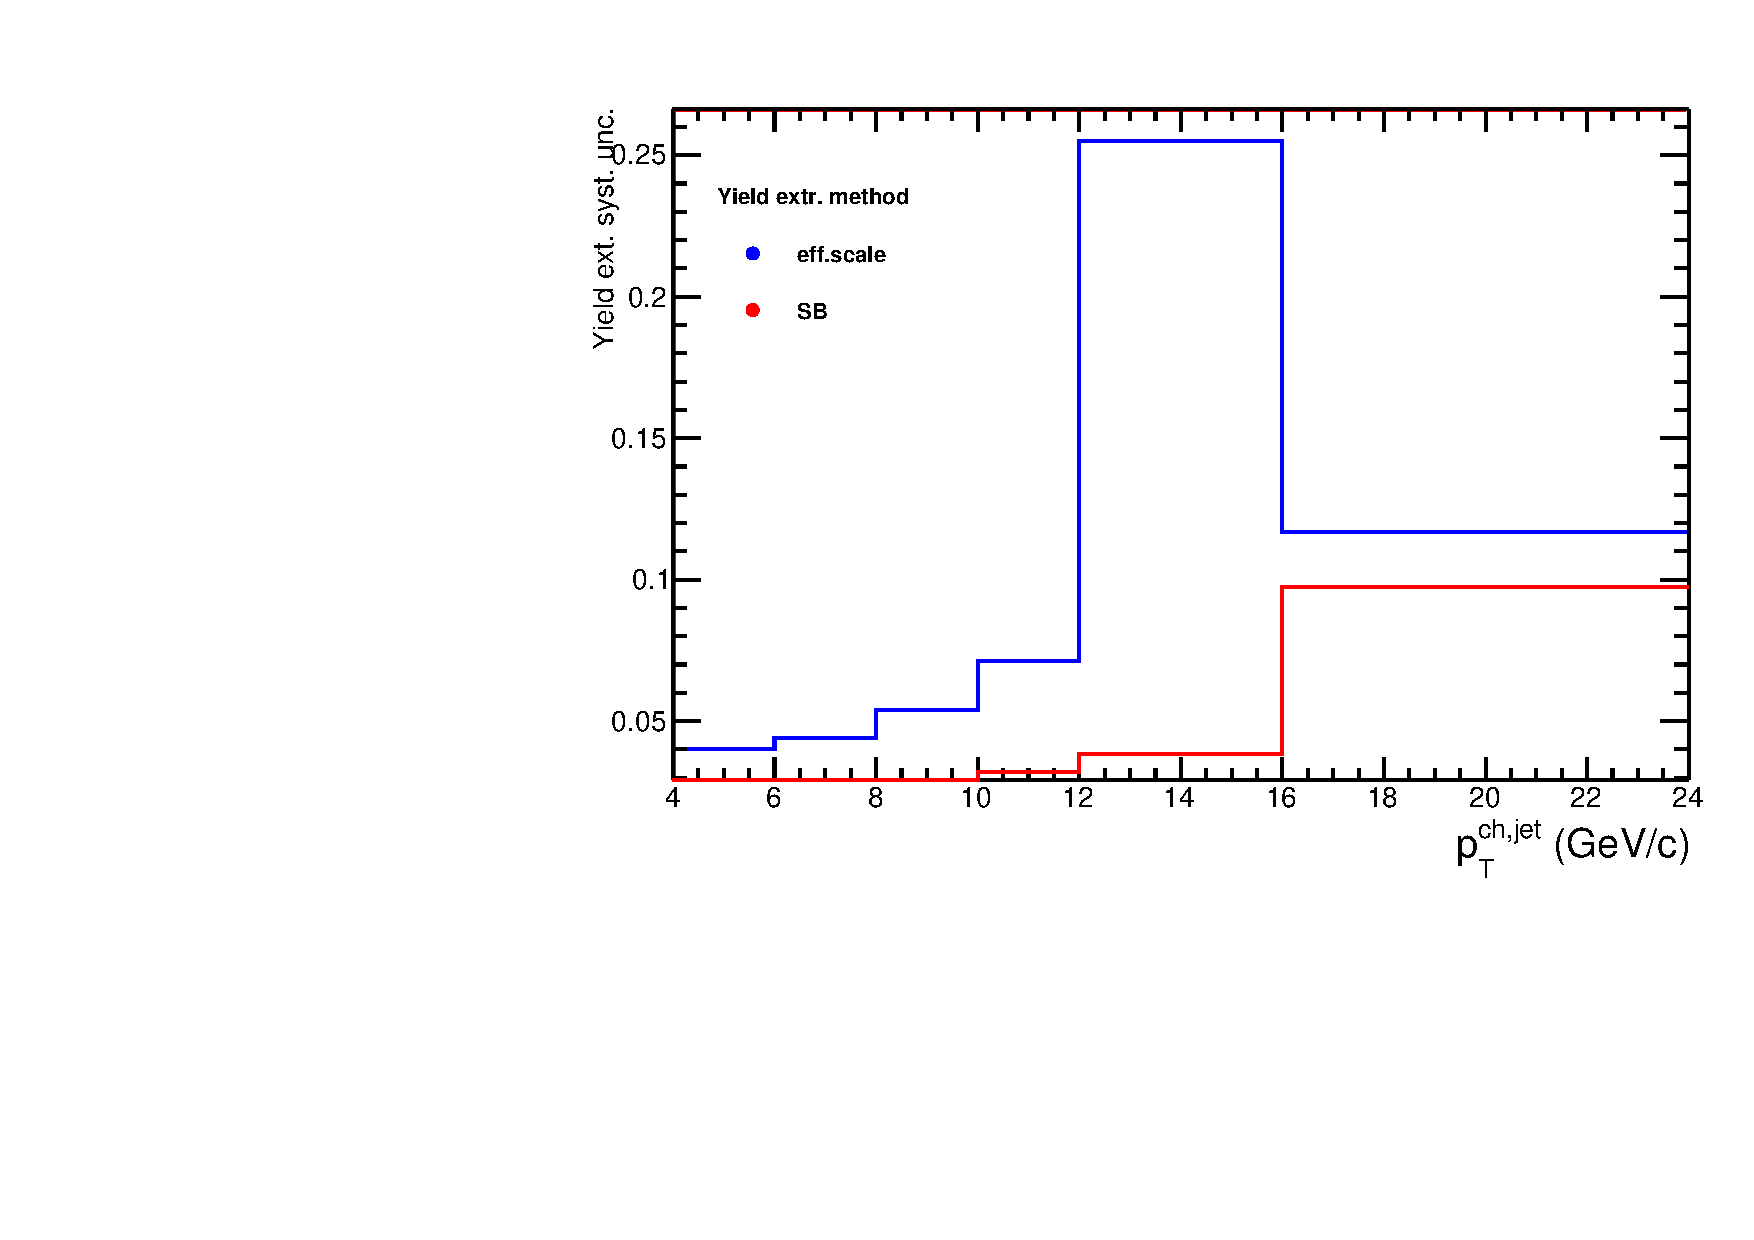
\includegraphics[width=0.95\linewidth]{img/rawYieldpPb/YieldExtSysUnc.pdf}
\end{minipage}
	
\end{columns}
\end{frame}

\subsection{Response Matrix \& Unfolding}

\begin{frame}{Response matrices}
\begin{overpic}[width=\textwidth, trim=0 40 0 70, clip]{img/DJetspPb_1}
\end{overpic}
\end{frame}

\begin{frame}{Quick look at unfolding with combined matrix}
\begin{center}
\begin{overpic}[width=.9\textwidth, trim=0 0 0 70, clip]{img/DJetspPb_2}
\end{overpic}
\end{center}
\end{frame}

\section{Summary}

\begin{frame}{Fully corrected spectrum for \pp\ at $\s=7$~TeV}
\begin{columns}
\column{.50\textwidth}
\begin{overpic}[width=\textwidth, trim=0 0 0 0, clip]{img/TheoryComparison_powheg_Charged_R040_1478868679_LHC10_Train823_LHC15i2_Train961_efficiency}
\end{overpic}
\column{.50\textwidth}
\begin{overpic}[width=\textwidth, trim=0 0 0 0, clip]{img/TheoryComparison_powheg_Charged_R040_1478868679_LHC10_Train823_LHC15i2_Train961_efficiency_Ratio}
\end{overpic}
\end{columns}
\begin{itemize}
\item \Dzero-jets in \pp\ collisions at $\s=7$~TeV
\item Raw yield extracted with the invariant mass fit in \ptchjet\ bins
\item B feed-down subtracted using a POWHEG+PYTHIA simulation
\item Unfolded using Bayesian method
\item Hint at \textbf{larger yield} in data compared to POWHEG+PYTHIA6 (Perugia-2011)
\end{itemize}
\end{frame}

\begin{frame}{D mesons vs. FONLL}
\begin{columns}
\column{.50\textwidth}
\begin{overpic}[width=\textwidth, trim=300 500 70 50, clip]{img/1205_6344v1_p9}
\end{overpic}
\column{.50\textwidth}
\begin{itemize}
\item \href{https://doi.org/10.1007/JHEP10(2012)137}{Cacciari et al, Theoretical predictions for charm and bottom production at the LHC, JHEP 10 (2012) 137}
\item D meson spectra are in the upper band of FONLL calculations
\item Similarly as observed in \Dzero-jet compared with POWHEG+PYTHIA
\end{itemize}
\end{columns}
\end{frame}

\begin{frame}{\pp\ at $\s=7$~TeV vs. \pPb\ at $\snn=5.02$~TeV}
\begin{columns}
\column{.50\textwidth}
\begin{overpic}[width=\textwidth, trim=0 0 0 0, clip]{img/pPbComparison_Charged_R040_LHC10_Train823_LHC15i2_Train961_efficiency}
\end{overpic}
\column{.50\textwidth}
\begin{overpic}[width=\textwidth, trim=0 0 0 0, clip]{img/pPbComparison_Charged_R040_LHC10_Train823_LHC15i2_Train961_efficiency_Ratio}
\end{overpic}
\end{columns}
\begin{itemize}
\item Note: B feed-down correction applied for \pp\ but not for \pPb\ (about 20\% in \pp)
\end{itemize}
\end{frame}

\begin{frame}{Conclusions}
\begin{itemize}
     \item \pp\ Analysis
    \begin{itemize}
        \item First fully corrected \pt\ spectrum of c-jets tagged using \Dzero\ mesons
        \item Systematics:
        \begin{itemize}
            \item Unfolding: uncertainty negligible (much smaller than statistical uncertainty)
            \item B feed-down: variations of PDF, $m_{\rm b}$, $\mu_0$, $\mu_F$, $\mu_R$ (time scale: first estimate $\sim$~10 days, finalized by preview week)
            \item Raw yield extraction: in progress (time scale: 2-3 days)
            \item Cut variations: some stability checks needed, can use most of the work done for D meson spectra (time scale: 1 week)
        \end{itemize}
    \end{itemize}
    \item \pPb\ Analysis
    \begin{itemize}
        \item B feed-down needs to be done
        \item Systematics:
        \begin{itemize}
            \item Unfolding: in progress (2-3 days)
            \item Raw yield extraction: under finalization (time scale: 2-3 days)
        \end{itemize}
    \end{itemize}
\end{itemize}
\end{frame}

\begin{frame}{Plans}
\begin{itemize}
\item First draft of the analysis note will be sent to the ARC tonight
\item Update in $\sim10$ days with finalized systematics
\item \pp\ Analysis: large statistical uncertainties $\approx 20-50$~\%
\begin{itemize}
\item First measurement with minimum-bias collisions $\rightarrow$ short paper
\end{itemize}
\item Looking forward to analyze the available statistics from both Run-1 and Run-2, including EMCal triggered data!
\end{itemize}
\end{frame}

\section*{Extra}

\begin{frame}{Extra Slides}
\huge
\begin{center}
Extra Slides
\end{center}
\end{frame}

\subsection*{Raw Yield Extraction}

\begin{frame}{Side-Band Spectra}
\begin{center}
\begin{overpic}[width=.85\textwidth, trim=0 0 0 0, clip]{img/D0_Charged_R040_JetPtSpectrum_DPt_20_SideBand_BkgVsSig}
\end{overpic}
\end{center}
\begin{itemize}
\item \textcolor{BrickRed}{SB} jet spectra ($4\sigma_{\rm fit}<|m-m_{\rm fit}|<8\sigma_{\rm fit}$) \textcolor{ForestGreen}{subtracted} from \textcolor{NavyBlue}{peak region} ($|m-m_{\rm fit}|<2\sigma_{\rm fit}$)
\end{itemize}
\end{frame}

\begin{frame}{MC Closure Test}
\begin{columns}
\column{.50\textwidth}
\begin{overpic}[width=\textwidth, trim=0 0 0 0, clip]{img/MC_Charged_R040_JetPtSpectrum_DPt_20_SpectraComparison}
\end{overpic}
\column{.50\textwidth}
\begin{overpic}[width=\textwidth, trim=0 0 0 0, clip]{img/MC_Charged_R040_JetPtSpectrum_DPt_20_SpectraComparison_Ratio}
\end{overpic}
\end{columns}
\begin{itemize}
\item Spectra obtained using the inv. mass fit and SB methods compared with MC truth
\end{itemize}
\end{frame}

\begin{frame}{Comparison between Eff.Scale and SB}
\begin{overpic}[width=\textwidth, trim=0 80 0 30, clip]{img/DJetspPb_3}
\end{overpic}
\end{frame}

\begin{frame}{Systematic uncertainty from yield extraction}
\begin{center}
\begin{overpic}[width=.9\textwidth, trim=0 15 0 55, clip]{img/DJetspPb_4}
\end{overpic}
\end{center}
\end{frame}

\begin{frame}{Systematic uncertainty from yield extraction (cont'd)}
\begin{center}
\begin{overpic}[width=.9\textwidth, trim=0 25 0 55, clip]{img/DJetspPb_5}
\end{overpic}
\end{center}
\end{frame}

\begin{frame}{Systematic uncertainty from yield extraction}
\begin{center}
\begin{overpic}[width=.9\textwidth, trim=0 15 0 55, clip]{img/DJetspPb_7}
\end{overpic}
\end{center}
\end{frame}

\begin{frame}{Systematic uncertainty from yield extraction (cont'd)}
\begin{center}
\begin{overpic}[width=.9\textwidth, trim=0 15 0 55, clip]{img/DJetspPb_8}
\end{overpic}
\end{center}
\end{frame}

\begin{frame}{Systematic uncertainty from yield extraction (cont'd)}
\begin{center}
\begin{overpic}[width=.9\textwidth, trim=0 15 0 55, clip]{img/DJetspPb_9}
\end{overpic}
\end{center}
\end{frame}

\subsection*{Detector Performance}

\begin{frame}{Prompt vs. Non-Prompt Reconstruction Efficiency}
\begin{center}
\begin{overpic}[width=.7\textwidth, trim=0 0 0 0, clip]{img/ReconstructionEfficiencyComparison}
\end{overpic}
\end{center}
\vspace{-20pt}
\begin{itemize}
\item Efficiency is higher for b~$\rightarrow$~\Dzero\ because of the longer decay length of B mesons (topological cuts)
\end{itemize}
\end{frame}

\begin{frame}{Efficiency vs. \ptchjet\ and \ptd}
\begin{columns}
\column{.50\textwidth}
\begin{overpic}[width=\textwidth, trim=0 0 0 0, clip]{img/D0_Jet_AKTChargedR040_pt_scheme_JetPtDPtSpectrum_PartialEfficiency}
\end{overpic}
\column{.50\textwidth}
\begin{overpic}[width=\textwidth, trim=0 0 0 0, clip]{img/D0_Jet_AKTChargedR040_pt_scheme_JetPtDPtSpectrum_PartialEfficiencyRatios}
\end{overpic}
\end{columns}
\begin{itemize}
\item Reconstruction efficiency largely independent of \ptchjet, for $5<\ptchjet<30$~\GeVc
\end{itemize}
\end{frame}

\subsection*{Unfolding}

\begin{frame}{Bin-By-Bin Correction Factors}
\begin{center}
\begin{overpic}[width=.65\textwidth, trim=0 5 50 10, clip]{img/InvMassFit_DPt_20_BinByBinCorrectionFactors}
\end{overpic}
\end{center}
\vspace{-20pt}
\footnotesize
\begin{itemize}
\item Bin-By-Bin correction factors: ratio between particle-level and detector-level
\item Some dependence on the prior (= particle-level spectrum)
\item 5-15\% correction
\end{itemize}
\end{frame}

\begin{frame}{Method Comparison}
\begin{columns}
\column{.50\textwidth}
\begin{overpic}[width=\textwidth, trim=0 0 0 0, clip]{img/InvMassFit_DPt_20_UnfoldingMethod}
\end{overpic}
\column{.50\textwidth}
\begin{overpic}[width=\textwidth, trim=0 0 0 0, clip]{img/InvMassFit_DPt_20_UnfoldingMethod_Ratio}
\end{overpic}
\end{columns}
\begin{itemize}
\item Baseline: Bayesian
\item Compared with: bin-by-bin correction, regularized SVD
\item All methods give equivalent results within few \% (large statistical uncertainty!)
\end{itemize}
\end{frame}

\begin{frame}{Prior Choice (Bayesian)}
\begin{columns}
\column{.50\textwidth}
\begin{overpic}[width=\textwidth, trim=0 0 0 0, clip]{img/InvMassFit_DPt_20_UnfoldingPrior_Bayes}
\end{overpic}
\column{.50\textwidth}
\begin{overpic}[width=\textwidth, trim=0 0 0 0, clip]{img/InvMassFit_DPt_20_UnfoldingPrior_Bayes_Ratio}
\end{overpic}
\end{columns}
\begin{itemize}
\item Priors: PYTHIA spectrum, power laws index 3 and 7 (quite large variation)
\item $\rightarrow$ no effect on the unfolding
\end{itemize}
\end{frame}

\begin{frame}{Bayesian Regularization (iterations)}
\begin{columns}
\column{.50\textwidth}
\begin{overpic}[width=\textwidth, trim=0 0 0 0, clip]{img/InvMassFit_DPt_20_UnfoldingRegularization_Bayes_PriorResponseTruth}
\end{overpic}
\column{.50\textwidth}
\begin{overpic}[width=\textwidth, trim=0 0 0 0, clip]{img/InvMassFit_DPt_20_UnfoldingRegularization_Bayes_PriorResponseTruth_Ratio}
\end{overpic}
\end{columns}
\begin{itemize}
\item Very fast convergence
\item Stable after 3 iterations, then $< 1$\% variations
\end{itemize}
\end{frame}

\begin{frame}{Priors}
\begin{columns}
\column{.50\textwidth}
\begin{overpic}[width=\textwidth, trim=0 0 0 0, clip]{img/InvMassFit_DPt_20_Priors}
\end{overpic}
\column{.50\textwidth}
\begin{overpic}[width=\textwidth, trim=0 0 0 0, clip]{img/InvMassFit_DPt_20_Priors_Ratio}
\end{overpic}
\end{columns}
\begin{itemize}
\item PYTHIA6 spectrum
\item Power-law spectra: $\ptjet^{-a}$, with $a=3, 7$
\end{itemize}
\end{frame}

\begin{frame}{MC Unfolding Closure Test: Signal-Only Spectra}
\begin{columns}
\column{.50\textwidth}
\begin{overpic}[width=\textwidth, trim=0 0 0 0, clip]{img/MC_SignalOnly_DPt_20_UnfoldingMethod}
\end{overpic}
\column{.50\textwidth}
\begin{overpic}[width=\textwidth, trim=0 0 0 0, clip]{img/MC_SignalOnly_DPt_20_UnfoldingMethod_Ratio}
\end{overpic}
\end{columns}
\begin{itemize}
\item Detector-level spectra obtained (signal-only via MC truth info) are unfolded and compared with the MC generated spectra
\end{itemize}
\end{frame}

\begin{frame}{MC Unfolding Closure Test: Inv.Mass Fit Spectra}
\begin{columns}
\column{.50\textwidth}
\begin{overpic}[width=\textwidth, trim=0 0 0 0, clip]{img/MC_InvMassFit_DPt_20_UnfoldingMethod}
\end{overpic}
\column{.50\textwidth}
\begin{overpic}[width=\textwidth, trim=0 0 0 0, clip]{img/MC_InvMassFit_DPt_20_UnfoldingMethod_Ratio}
\end{overpic}
\end{columns}
\begin{itemize}
\item Spectra obtained using the inv. mass fit are unfolded and compared with the MC generated spectra
\end{itemize}
\end{frame}


\end{document}
